\chapter{Introduction to Hamiltonian Systems}
A canonical Hamiltonian system is given by two state variables $p,q \in \mathbb{R}^{n}$ (i.e. the entire system is even dimensional), a \emph{Hamiltonian} function $H(p,q,t)\in \mathcal{C}^{1}(\mathbb{R}^{2n}\times \mathbb{\mathbb{R}})$ which maps $\mathbb{R}^{n}\times\mathbb{R}^{n}\times\mathbb{R}\to \mathbb{R}$. In general $q$ denotes the generalized coordinates (position) and $p$ the generalized momenta. The dynamics on the system is given by
\begin{align}
	\begin{dcases}
		\dot{q} = \frac{\partial H(q,p,t)}{\partial p}\\
		\dot{p} = - \frac{\partial H(q,p,t)}{\partial q}.
	\end{dcases}
\end{align}
This is represented in shorthand notation by using the identity matrix, denoted by $I_{n}\in\mathbb{R}^{n\times n}$ and the symplectic matrix
\begin{align}
	J = 
	\begin{pmatrix}
		0 & I_{n}\\
		-I_{n} & 0
	\end{pmatrix}
.	
\end{align}
Denote the differential with respect to the state variables $x =
\begin{pmatrix}
	p \\ q
\end{pmatrix}
\in \mathbb{R}^{2n}$ by
\begin{align}
	D_{x} = D = 
	\begin{pmatrix}
		\frac{\partial}{\partial q} \\
		\frac{\partial}{\partial p}
	\end{pmatrix}
.	
\end{align}
Then the shorthand notation for the system is
\begin{align}
	\boxed{
	\dot{x} = JD_{x}H(x,t).
}
\end{align}

\begin{ex}[Holonomic mechanical systems are Hamiltonian]
	Assume that all external forces are derived from a potential, i.e. $F(q,t)= -\frac{\partial V(q,t)}{\partial q}$ where $q$ denotes the position. Further assume that all constraints are geometric, i.e. $f(q,t)=0$. We have $n$ degrees of freedom as $q \in \mathbb{R}^{n}$ and $\dot{q} \in \mathbb{R}^{n}$. The kinetic energy is given by $T(q,\dot{q})$ and the potential energy by $V(q,t)$. We then use the principle of least action (also referred to as Hamilton's principle) to derive the equations of motion. This can be shown to be equivalent to Newton's second law. This principle states that for the \emph{Lagrangian} $L(q, \dot{q}, t) = T(q,\dot{q})-V(q,t)$ we have that the variation of the action $S$ is 0
	\begin{align}
		\boxed{
		\delta S = \delta \int_{t_0}^{t_1} L(q(s), \dot{q}(s), s)ds = 0. \numberthis \label{eq8:ELE} 
	}
	\end{align}
	This implies the \emph{Euler-Lagrange equations}
	\begin{align}
\frac{d}{dt} \frac{\partial L}{\partial \dot{q}} - \frac{\partial L}{\partial q} = 0.	
	\end{align}
Thus we have $n$, second-order ODEs. 

\begin{remark}[]
	In \eqref{eq8:ELE} the variation $\delta S$ being equal to 0 stems from the principle of least action, as the action $\int_{}^{} L(q(s), \dot{q}(s), s)ds$ is then a minimum. The variational of a function $\delta F$ (here $F[\gamma]=\int_{}^{} \gamma ds)$ of a path (in our case $\gamma = (q(s), \dot{q}(s), s)$) corresponds to seeing how infinitesimal changes to the path change the output of the functional. These different, admissible paths are depicted in Fig. \ref{fig:variational_deriv}. Hamilton's principle states that among these different paths the one that will physically take place is the one along which the action $S$ is minimal.
	\begin{figure}[h!]
		\centering
		\includegraphics[width=0.5\textwidth]{figures/ch8/1variational_deriv.pdf}
		\caption{An illustration of various different paths (denoted here by $q(t)$). The red demarcates the actual motion which occurs in the system, whereas the green paths are each admissible motions which are consistent with the constraints.}
		\label{fig:variational_deriv}
	\end{figure}
\end{remark}
Now assume that $L$ is a convex function of $\dot{q}$. Using this the \emph{Legendre transfomation} of $L$ can be performed, which is essentially just a different way to look at the graph of $L(q, \cdot, t)$. This transformation gives us
\begin{align}
	\boxed{H\left(q, \frac{\partial L}{\partial \dot{q}}, t\right) = \frac{\partial L}{\partial \dot{q}}\dot{q} - L(q, \dot{q}, t).} \label{eq8:hamiltonian_def}
\end{align}
Th geometric interpretation of this is shown in Fig. \ref{fig:legendre_trafo}. At each velocity $\dot{q}$ the tangent line of $L(q, \cdot, t)$ is taken and shifted such that the $y$-intercept is at $0$. Then $H$ is equal to the difference between this shifted line and the function $L(q, \dot{q}, t)$.
\begin{figure}[h!]
	\centering
	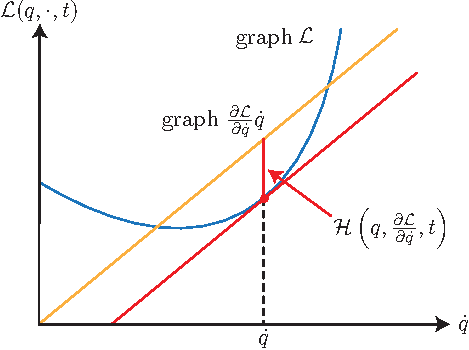
\includegraphics[width=0.5\textwidth]{figures/ch8/2legendre_trafo.pdf}
	\caption{The Legendre transformation. The thin red linear function denotes the tangent of $L(q, \cdot, t)$ taken at  $\dot{q}$, the yellow linear function is then the shifted version with a 0 $y$-intercept, and the thick red vertical line is the Legendre transformation $H$ measuring the difference between this shifted line and $L(q,\cdot, t)$.}
	\label{fig:legendre_trafo}
\end{figure}

As $L$ is convex, if we define the generalized momenta $p=\frac{\partial L}{\partial \dot{q}}$. There then exists a unique $\dot{q}$ such that $\dot{q} = F(q,p,t)$, in fact the relationship between $\dot{q}$ and $p$ here is bijective. We then have
\begin{align}
	H(q,p,t) = p F(q,p,t) - L (q, F(q,p,t), t)
\end{align}
the Hamiltonian associated with $L$ (or the Legendre transform of $L$).

At this point note that the total differential of $H(q,p,t)$ is
\begin{subequations}
\begin{align}
	dH &= \frac{\partial H}{\partial q}dq + \frac{\partial H}{\partial p}dp + \frac{\partial H}{\partial t}dt \\
	   &= d(pF) - \underbrace{\frac{\partial L}{\partial q}}_{=\dot{p}} dq - \underbrace{\frac{\partial L}{\partial \dot{q}}}_{=p} - \frac{\partial L}{\partial t}dt \\
	   &= \underbrace{F}_{=\dot{q}}dp + pdF - \dot{p}dq - pdF - \frac{\partial L}{\partial t}dt \\
	   &= \dot{q}dp - \dot{p}dq - \frac{\partial L}{\partial t}dt.
\end{align}
\end{subequations}
Comparing coefficients in the first and last equations then yields
\begin{align}
	\begin{dcases}
		\dot{q} = \frac{\partial H}{\partial p}\\
		\dot{p} = -\frac{\partial H}{\partial q}
	\end{dcases}
.	
\end{align}
This first-order ODE is called the \emph{Hamiltonian equations of motion}. The physical meaning of the Hamiltonian can be seen by substituting $L = T(q,\dot{q}) - V(q, t)$ into the definition \ref{eq8:hamiltonian_def}. The kinetic energy only depends on $\dot q$ through the kinetic energy, 
\begin{align}
\dot{q}\frac{\partial L}{\partial \dot{q}} = \dot{q} \frac{\partial T}{\partial \dot{q}}.
\end{align}
Since the kinetic energy is quadratic in the velocity, this simplifies to 
\begin{align}
\dot{q} \frac{\partial T}{\partial \dot{q}} = 2T(q,\dot{q}).
\end{align}
We then have 
\begin{align}
H = 2T - (T - V) = T(q, p) + V(q,t),
\end{align}
which is the full mechanical energy. Also note that we have $\frac{\partial H}{\partial t} = - \frac{\partial L}{\partial t}$.
\end{ex}

We will now apply this result to a well known system.

\begin{ex}[The Hamiltonian of the pendulum]
	Recall that for the pendulum the position is given by $q=\varphi\in S^{1}$, with a string of length $\ell$ the vertical deflection of the pendulum is $\ell(1- \cos(\varphi)$. The string is assumed massless and the mass at the end of the string is given by $m$. 
	
	We have the kinetic and potential energies
	\begin{align}
		T = T(\dot{q}) = \frac{1}{2} m (\ell \dot{\varphi})^{2} = \frac{1}{2} m\ell^2 \dot{\varphi}^{2};\quad V = V(q) = mg\ell(1-\cos(\varphi)).
	\end{align}
Therefore the Lagrangian is given by
\begin{align}
	L = T-V = \frac{1}{2}m \ell^2 \dot{\varphi}^{2} - mg\ell(1-\cos(\varphi)).
\end{align}
To find the generalized momentum, we calculate the partial derivative of the Lagrangian with respect to $\dot{q}$, i.e.
\begin{align}
p = \frac{\partial L}{\partial \dot{q}} = \frac{\partial L}{\partial \dot{\varphi}} = m\ell^2 \dot{\varphi}\implies \dot{\varphi} = \frac{p}{m\ell^2}.
\end{align}
Now it is possible to calculate the Hamiltonian
\begin{align}
	H = p \frac{p}{m\ell^2} - \frac{1}{2}m\ell^2 \frac{p^2}{(m\ell^2)^2} + mg\ell(1-\cos(\varphi))
	= \underbrace{\frac{1}{2} \frac{p^2}{m\ell^2}}_{T} + \underbrace{mg\ell(1-\cos(\varphi))}_{V}.
\end{align}
Hence for this Hamiltonian system we have the Hamiltonian equations of motion
\begin{align}
\begin{dcases}
	\dot{\varphi} = \frac{\partial H}{\partial p} = \frac{p}{m\ell^2} \\
	\dot{p} = - \frac{\partial H}{\partial q} = -mg\ell \sin (\varphi).
\end{dcases}
\end{align}
\end{ex}

\begin{exercise}
	Derive the Hamiltonian equations of motion for a the coupled pendulums shown in Fig. \ref{fig:ex81coupled_pendula}. (The two point masses $m$ are placed at the tips of two massless rods of length $L$. Both joints are frictionless; the constant of gravity is $g$.)
\begin{figure}[h]
\begin{centering}
	\includegraphics[width=0.4\textwidth]{figures/ch8/Series/coupledpendula.pdf}
	\label{fig:ex81coupled_pendula}
	\caption{Coupled system of two pendulums.}
\par\end{centering}
\end{figure}
	
\end{exercise}
\notebookbox{
\begin{notebook}
\href{https://drive.google.com/file/d/1fo84abyC_UBdkoHbNugs4-Ak6WfoxE0-/view?usp=sharing}{Derivation of the equations of motion of the double pendulum.}
\end{notebook}
}

\begin{ex}[2-dimensional incompressible fluids are Hamiltonian]
	We begin on a domain $\mathcal{D}$ contained on the plane which is simply connected, i.e. it has no holes. For each position $x\in \mathcal{D}$ we have the velocity field
	\begin{align}
		{V}(x,t) = 
		\begin{pmatrix}
			u(x,y,t) \\ v(x,y,t)
		\end{pmatrix},
	\end{align}
	i.e. for each position we have
	 \begin{align}
		\begin{pmatrix}
			\dot{x} \\ \dot{y}
		\end{pmatrix}
		= 
		\begin{pmatrix}
			u \\v
		\end{pmatrix}
		.
	\end{align}
This is depicted in \ref{fig:incompressible}.
\begin{figure}[h!]
	\centering
	\includegraphics[width=0.5\textwidth]{figures/ch7/2_5simply_connected.pdf}
	\caption{The simply connected domain $\mathcal{D}$ with the velocity field $V$.}
	\label{fig:incompressible}
\end{figure}

The incompressibility condition is given by 
\begin{align}
	\nabla \cdot V = \frac{\partial u}{\partial x} + \frac{\partial v}{\partial y}= 0\quad \forall x\in \mathcal{D}\subset \mathbb{R}^{2}. \label{eq8:incompressibility}
\end{align}
Now rewrite \eqref{eq8:incompressibility} in terms of a three dimensional vector field as
\begin{align}
	\nabla \times 
	\begin{pmatrix}
		-v \\ u \\ 0 
	\end{pmatrix}
	=0 \Leftrightarrow
	\nabla \cdot V = 0.
\end{align}
The third component is calculated as $\frac{\partial u}{\partial x} - \frac{\partial (-v)}{\partial y} = \frac{\partial u}{\partial x} + \frac{\partial v}{\partial y} = 0$. On $\mathcal{D}\times \mathbb{R}$ (which is simply connected in $\mathbb{R}^{3}$) the vector field $
\begin{pmatrix}
	-v \\ u \\ 0
\end{pmatrix}
$ has zero curl. Therefore there exists a potential of this vector field $\Psi:\mathcal{D}\times \mathbb{R} \to \mathbb{R}$ such that
\begin{align}
\begin{pmatrix}
	-v \\ u \\ 0 
\end{pmatrix}
 = \nabla \Psi =
 \begin{pmatrix}
 	\partial_x \Psi \\ \partial_y \Psi \\ \partial_z \Psi
 \end{pmatrix}.
\end{align}
Because of the third equation $\Psi$ has no z dependence and we can write our potential as $\Psi = \Psi(x, y, t)$. Therefore we find
\begin{align}
	\begin{dcases}
		-\dot{y} = \frac{\partial \Psi}{\partial x} \\
		\dot{x} = \frac{\partial \Psi}{\partial y}
	\end{dcases}
	\implies 
	\begin{dcases}
		\dot{x} = \frac{\partial \Psi(x,y,t)}{\partial y} \\
	\dot{y} = -\frac{\partial \Psi(x,y,t)}{\partial x}.
	\end{dcases}
\end{align}
Thus we have shown that particle motion is Hamiltonian.
\end{ex}

\begin{exercise}
Consider a two-dimensional steady \emph{compressible} fluid flow with velocity field ${v(x})=\left(u(x,y),v(x,y)\right)$, where ${x}=\left(x,y\right)$. Assume that the flow conserves mass, i.e., its density function $\rho\left({x}\right)>0$ satisfies the equation of continuity. The latter equation, in its general form for unsteady flows, reads 
\begin{align}
\rho_{t}+\nabla\cdot\left(\rho{v}\right)=0,
\end{align}
valid or general, unsteady flow. Show that the equation of fluid particle motion becomes a canonical Hamiltonian system after a rescaling of time.
\end{exercise}

\begin{ex}[Planar, autonomous dynamical systems with a conserved quantity are Hamiltonian]
	We begin with the dynamical system which has a first integral $U$ (which is not constant), i.e.
	\begin{align}
		\dot{x} = f(x);\quad x \in \mathbb{R}^{2};\quad \exists U:\mathbb{R}^{2}\to \mathbb{R}:\ \frac{dU(x(t))}{dt}=0.
	\end{align}
	Note that this first integral property has further implications
	\begin{align}
		\frac{dU(x(t))}{dt} = DU(x(t)) \cdot \dot{x}(t) = DU \cdot \left.f\right|_{x(t)} = 0 \implies DU \perp f.
	\end{align}
Therefore, we can take the orthogonal complement of $DU$ and scale this to be equal to $f$, i.e.
\begin{align}
	f(x) = p(x) JDU(x) \implies \dot{x} = p(x) JDU(x).
\end{align}
Such a system is called a \emph{generalized Hamiltonian system} with the scalar function $p(x)$. Here the symplectic matrix in 2 dimensions is given by the $90^{\degree}$ rotation
\begin{align}
	J = 
	\begin{pmatrix}
		0 & I_{1}\\
		-I_{1} & 0 
	\end{pmatrix}
	=
	\begin{pmatrix}
		0 & 1 \\
		-1 & 0
	\end{pmatrix}
	.
\end{align}
If we assume $p(x)\neq0$ for all $x\in \mathcal{D} \subset \mathbb{R}^{2}$ then we may define the trajectory-dependent rescaling of time
\begin{align}
	\tau = \int_{0}^{t} p(x(s))ds.
\end{align}
Then, define the notation for the derivative with respect to $\tau$ as follows
 \begin{align}
	 \frac{d(\ )}{dt} = \frac{d(\ )}{d\tau} \underbrace{\frac{d\tau }{dt}}_{p(x(t))} = (\ )' p.
\end{align}
Hence, using this time-transformation we have
\begin{align}
	\dot{x} = pJDU \implies x'p = pJDU \implies \boxed{x' = JDU(x).}
\end{align}
Therefore, we have a canonical Hamiltonian system. In fact, all planar, autonomous systems with a nontrivial first integral are Hamiltonian systems after a possible reparameterization of time.
\end{ex}

\begin{remark}[]
	The fact that the first integral was not trivial (i.e. non-constant) is critical, as otherwise $DU$ would be constantly 0, as we must be able to phrase the right hand side $f$ in terms of $DU$. Only in the case $f=0$ would this then be possible.
\end{remark}

\begin{ex}[Lotka-Volterra model (1925) for predator-prey interactions]
	For more information about this model see \cite{Lotka1925, Volterra1926}. Let the size of the prey population be represented by $h(t)$ and the size of the predator population be denoted by $p(t)$. Each of these populations must be at least 0. Now for strictly positive constants $a_1$, $a_2$, $b$, and $c$ we have the following dynamics
	\begin{align}
		\begin{dcases}
			\dot{h} = a_1 h(1- bp) \\
			\dot{p} = -a_2 p(1-ch).
		\end{dcases}
	\end{align}
	The phase portrait of this system is depicted in Fig. \ref{fig:lotka_volterra}.
	\begin{figure}[h!]
		\centering
		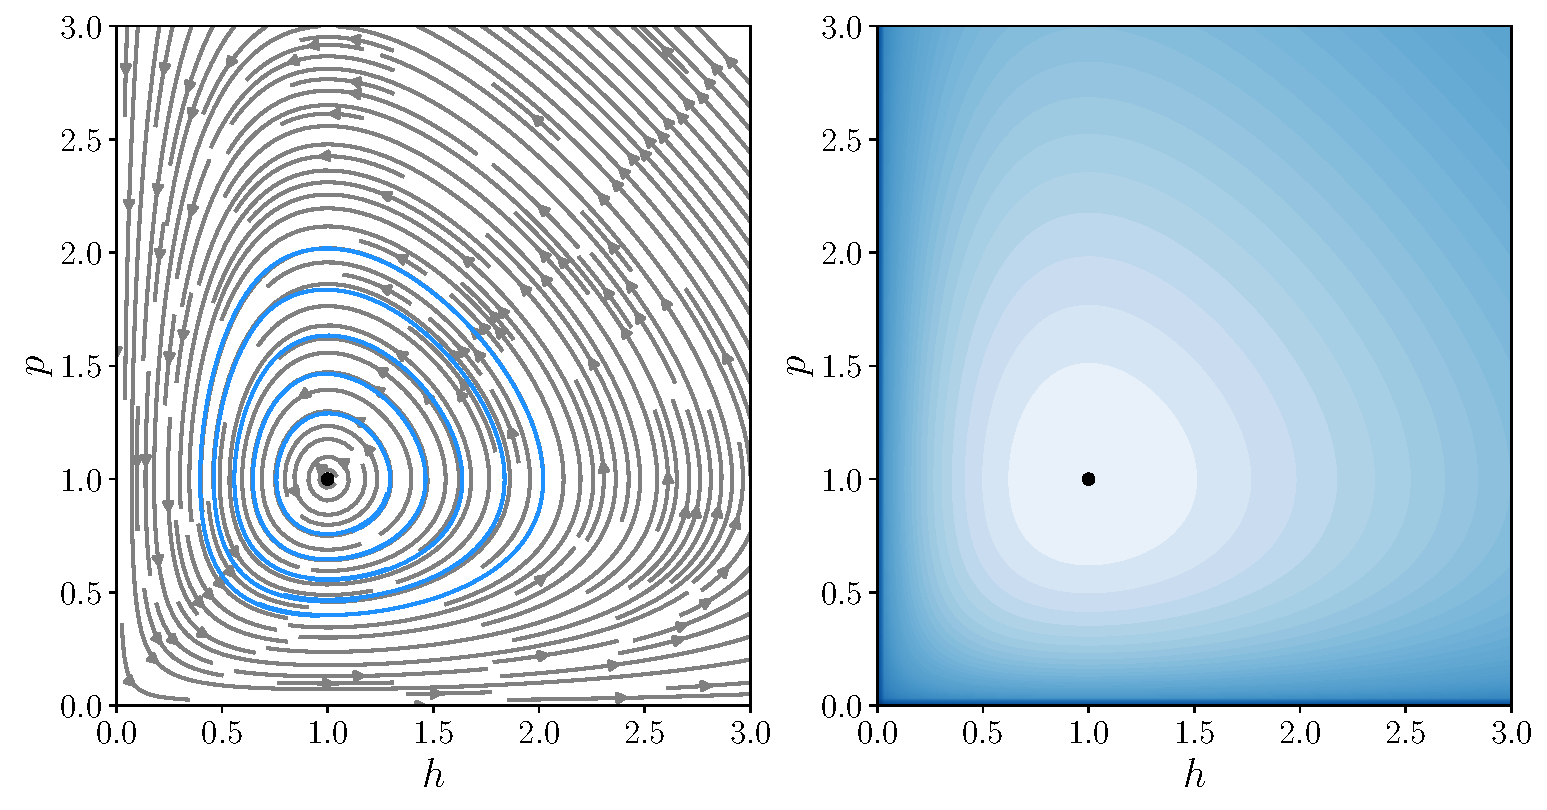
\includegraphics[width=0.5\textwidth]{figures/ch8/3lotka_volterra.pdf}
		\caption{The phase portrait of the Lotka-Volterra dynamics, which has been used to explain the observed cycles in fish populations.}
		\label{fig:lotka_volterra}
	\end{figure}

	This system does in fact have a first integral, and thus it is Hamiltonian.	
\end{ex}

Now that we have seen multiple examples of Hamiltonian systems, we would like to better understand what properties they all share.

\begin{exercise}
Consider a dynamical system defined on the two-dimensional torus $\mathbb{T}^{2}=\mathcal{S}^{1}\times \mathcal{S}^{1}$.
Such systems admit the general form
\begin{align}
\dot{\phi}_{1} & =  a(\phi_{1},\phi_{2})\\
\dot{\phi}_{2} & =  b(\phi_{1},\phi_{2}),\label{eq:ex83_2}
\end{align}
where $\phi_{i}\in \mathcal{S}^{1}$.

\begin{enumerate}
	\item Show that a physical example of system \eqref{eq:ex83_2} is found in
the motion of two uncoupled linear undamped oscillators. Specifically,
show that orbits of 
\begin{align}
\ddot{x}+x & =  0\\
\ddot{y}+y & =  0,
\end{align}
are confined to two-dimensional invariant tori of the phase space.

\item Assume that system \eqref{eq:ex83_2} has no fixed point (which is the
	case in the oscillator example). Argue that \eqref{eq:ex83_2} then \emph{cannot}
be Hamiltonian, even after a rescaling of time. (\emph{Hint:} Use
the fact that a continuous function defined on a compact set must
have a minimum and a maximum). 
\end{enumerate}
\end{exercise}

\begin{exercise}
Show that for any dynamical system $\dot{q}=f(q,t)$, $q\in\mathbb{R}^{n}$, one can select a canonically conjugate variable $p\in\mathbb{R}^{n}$, such that the evolution of $(q(t),p(t))$ is governed by a Hamiltonian system. (Thus any type of dynamics can be viewed as a projection from a higher-dimensional Hamiltonian dynamical system.)	
\end{exercise}


\section{Properties of Hamiltonian systems}
The setup going forward will be as follows for $n\geq 1$
\begin{align}
	\dot{x} = JDH(x,t);\quad x=
	\begin{pmatrix}
		q \\ p
	\end{pmatrix}
	\in \mathbb{R}^{2n};\quad 
	J=
	\begin{pmatrix}
		0 & I_n\\
		-I_n & 0 
	\end{pmatrix}.\numberthis \label{eq8:hamiltonian}	
\end{align}
\begin{proposition}[Conservation of the Hamiltonian (energy)]
	If $\frac{\partial H}{\partial t}=0$ (i.e. $H$ is only a function of $q$ and $p$) then $H(x(t))$ is constant on all trajectories. Therefore $H(x)$ is a first integral.	
\end{proposition}
\begin{proof}
	Use $J = -J^{T}$ to calculate
	\begin{align}
		\frac{dH(x(t))}{dt} = DH(x(t)) \cdot JDH(x(t)) = \left.\langle DH, JDH \rangle \right|_{x= x(t)} = 0.
	\end{align}
\end{proof}
The \emph{energy surface} for some constant $E_{0}=\left\{ x \in \mathbb{R}^{2n}:\ H(x)= H_0 \right\} $, for some constant $H_0$, is an invariant surface for the system. By nature of this $JDH$ must be tangent to $E_0$. Assuming that $E_0$ contains no fixed points of \eqref{eq8:hamiltonian} is equivalent to $DH(x_0)\neq 0$ for all $x_0$ in $E_0$. Hence, by the Implicit Function Theorem, the solution of $H(x)-H_0=0$ can be smoothly continued from $x_0$. Indeed, we have
\begin{align}
	DH(x_0)\neq 0\in \mathbb{R}^{2n} \implies \exists i:\ \left.\frac{\partial H}{\partial x^{i}}\right|_{x=x_0} \neq 0.
\end{align}
Then we have $x^{i}=F\left(x^{1},\ldots,x^{i-1},x^{i+1},\ldots,x^{2n}\right)$ for $F\in \mathcal{C}^{1}$, because $H$ is smooth. This implies that $E_{0}$ is a smooth $2n-1$-dimensional graph (i.e. a smooth hypersurface or codimension-one surface).

\begin{ex}[Two degree of freedom nonlinear oscillator]
	Between two fixed sides, three nonlinear springs hold two masses. Each spring has a potential given by $V_{i}$ for $i=1,2,3$ and the masses are given by $m_1$ and $m_2$. The displacement of each mass is given by $q_1$ and $q_2$ respectively. The potentials have global minima at $x=(q_1, q_2)^T=0$, and are otherwise strictly monotone. The system and example potential are illustrated in Fig. \ref{fig:2dof_oscillator_hamiltonian}.
	\begin{figure}[h!]
		\centering
		\includegraphics[width=0.5\textwidth]{figures/ch8/4_2dof_oscillator_hamiltonian.pdf}
		\caption{The two degree of freedom nonlinear oscillator and an example of a potential $V_i$.}
		\label{fig:2dof_oscillator_hamiltonian}
	\end{figure}
	
	For this system the specific conditions on the potentials are
	\begin{align}
		V_{i}(0) =0;\quad V_{i}'(0)=0;\quad V_{i}''(0)>0;\quad \forall x\neq 0:\ V_{i}''(x)\neq 0 . \label{eq8:2dof_conditions}
	\end{align}

	The Lagrangian is then
	\begin{align}
		L=T-V = \frac{1}{2} m_1 \dot{q}_{1}^{2} + \frac{1}{2}m_2 \dot{q}_{2}^{2} - \left[V_1(q_1) + V_2(q_2 - q_1) + V_3(-q_2) \right].
	\end{align}
From the Lagrangian the generalized momenta can be derived
\begin{align}
	p_i = \frac{\partial L}{\partial \dot{q}_{i}} = m_{i} \dot{q}_{i} \implies \dot{q}_{i} = \frac{p_i}{m_i}\quad i=1,2.
\end{align}
And with this the Hamiltonian can be calculated as
\begin{align}
	H = T+V = \frac{1}{2}\frac{p_1^{2}}{m_1} + \frac{1}{2}\frac{p_{2}^{2}}{m_{2}} + V_1(q_1) + V_2(q_2 - q_1) +V_{3}(-q_2).
\end{align}
Now recall that $\dot{x}=JDH(x)$, therefore the fixed point $x_0=(q^{0}, p^{0})^{T}$ can be found by identifying the roots of $DH$ 
\begin{align}
	DH(x_0)=0 \Leftrightarrow
	\begin{pmatrix}
		V_{1}'(q_{1}^{0}) - V_{2}'(q_{2}^{0} - q_{1}^{0}) \\
		V_{2}'(q_{2}^{0} - q_{1}^{0}) - V_{3}'(-q_{2}^{0}) \\
		\frac{p_{1}^0}{m_1} \\
		\frac{p_{2}^{0}}{m_2}
	\end{pmatrix}.
\end{align}
For instance the origin is a fixed point, i.e.
\begin{align}
	x_0 = 
	\begin{pmatrix}
		q^{0} \\ p^{0}
	\end{pmatrix}
	=0\in \mathbb{R}^{4}.
\end{align}
Hence we have
\begin{align}
	p_{1}^{0} = p_{2}^{0}= 0;\quad V_{1}'(q_{1}^{0}) = V_{2}^{1}(q_2^{0}-q_{1}^{0});\quad V_{2}'(q_{2}^{0}-q_{1}^{0})=V_{3}'(-q_{2}^{0}) \label{eq8:2dof_star}.
\end{align}
Assume that $q_{1}^{0}>0$ solves \eqref{eq8:2dof_star}. Then we would have the following
\begin{align}
	V_{1}'(q_{1}^{0}) = V_{2}'(q_{2}^{0} - q_{1}^{0}) > 0 \implies q_{2}^{0}>q_{1}^{0} >0,
\end{align}
due to the conditions set out in \eqref{eq8:2dof_conditions}. However we also have that
\begin{align}
	V_{3}'(-q_{2}^{0}) = V_{2}'(q_{2}^{0}-q_{1}^{0})>0 \implies -q_{2}^{0}>0.
\end{align}
These two inequalities are clearly in contradiction. A similar argument shows that $q_{1}^{0} < 0$ also leads to a contradiction. Therefore we find that at all equilibria $q_{1}^{0}=0$ and by symmetry $q_{2}^{0}=0$ as well. Thus the only fixed point is given by $q_{1}^{0}=q_{2}^{0}=0$ and $p_{1}^{0}=p_{2}^{0}=0$. We can conclude that all nonzero energy surfaces are codimension-one (3-dimensional) invariant manifolds (i.e. smooth surfaces).

Now it is possible to analyze the stability of this fixed point. To use Lyapunov's direct method, the Hamiltonian is a good candidate for a Lyapunov function, because $H(0)=0$, $DH(0) = 0 \in \mathbb{R}^{4}$, and $\frac{dH(x(t))}{dt}=0$. We still need to find out if $H$ is cup shaped. First calculate the Hessian
\begin{align}
	D^2H = 
	\left(
	\begin{array}{c|c}
		D^2V & 0_{2\times 2} \\
		\hline
		0_{2\times 2} &
		\begin{array}{c c}
			\frac{1}{m_1} & 0 \\
			0 & \frac{1}{m_2}
		\end{array}
	\end{array}
\right)
.
\end{align}
Next, we evaluate if each of the diagonal matrices are positive definite. The lower right matrix is clearly positive definite as it is a diagonal matrix with strictly positive entries. For the upper left, a calculation is required
\begin{align}
\left.D^2V\right|_{0} = 
	\left.\begin{pmatrix}
		V_{1}'' + V_{2}'' & -V_{2}'' \\
		-V_{2}'' & V_{2}'' + V_{3}''
	\end{pmatrix} \right|_{x = 0 \in \mathbb{R}^{4}}.
\end{align}
Due to the fact that $\left. V_{1}'' + V_{2}''\right|_{0}>0$ and $\det\left(\left.D^2V\right|_{0}\right) >0$ we have that $\left.D^2V\right|_{0}$ is positive definite by Sylvester's theorem. Hence $D^2H$ is positive definite, i.e. cup shaped. Now we have shown that $H(x)$ is a Lyapunov function, and therefore guarantees that the origin is nonlinearly stable irrespective of the actual form of the potentials. 

From this we wonder what else can be said about the global phase space geometry, which leads us to the Morse lemma.
\begin{lemma}[Morse]
Let $x_0$ be a nondegenerate critical point for $f:\mathbb{R}^{n}\to \mathbb{R}$, i.e 
\begin{align}
	Df(x_0) =0,\quad \det\left(D^{2}f(x_0)\right)\neq 0.
\end{align}
Let $k$ be the number of negative eigenvalues of $D^2f(x_0)$. Then there exists a local change of coordinates (diffeomorphism) $x\mapsto y$ near $x_0 $ such that in the new coordinates
\begin{align}
	f(y) = f(x_0) - y_1^{2} - \ldots - y_{k}^{2} + y_{k+1}^{2} + \ldots +y_{n}^{2}.
\end{align}
\end{lemma}

By the Morse lemma, there exists a change of coordinates $x\mapsto y$ such that $H(y) = y_{1}^{2} + y_{2}^{2} + y_{3}^{2}+y_{4}^{2}$ that is suitable near the origin. Therefore the energy surface $E_{h_0} = \left\{ y \in \mathbb{R}^{4}:\ H(y) = h_0\right\}$ is equal to $\mathcal{S}^3 \subset \mathbb{R}^{4}$, where $\mathcal{S}^{3}$ is the 3-dimensional hyper-sphere. This means in the original $x$-coordinates, all low-energy level sets of $H(x)$ are diffeomorphic to $3$-dimensional spheres.
\end{ex}

It is possible to draw on other results from differential geometry, namely the foliation theorem \cite{Milnor1965}. This tells us that level surfaces of a scalar function can only change their topology (i.e. become no longer diffeomorphic to each other) through level surfaces that contain a critical point of the function ($Df$ must vanish somewhere on the level set). 

We can see this in the example of the pendulum equation, whose Hamiltonian we previously derived. The stable fixed point is a nondegenerate critical point of the Hamiltonian (as all other points around it have more energy) and by the Morse lemma, after a change of coordinates, level surfaces can be parametrized as a sum of quadratic terms. The loops representing periodic oscillation are also the level sets for the respective energy level and are all diffeomorphic to each other (they are all diffeomorphic to $\mathcal{S}^{1}$) until the level set which intersects the unstable fixed points. This transition is depicted in Fig. \ref{fig:morse_foliation}.

\begin{figure}[h!]
	\centering
	\includegraphics[width=0.5\textwidth]{figures/ch8/5morse_foliation.pdf}
	\caption{The effect of the foliation theorem. Around the stable fixed point where the Morse lemma applies is shaded orange, and the level sets containing critical points of $H$.}
	\label{fig:morse_foliation}
\end{figure}

Regarding the two degree of freedom oscillator example previously handled, all surfaces are diffeomorphic to $\mathcal{S}^{3}$ as $x=0$ is the only critical point of $H$.

\section{Volumes under Hamiltonian flow maps}
We would like to understand what happens with a volume of the phase space under the flow map of a Hamiltonian system. When we talk about the transformation of a volume $V(t_0)$ under the flow map, we mean to study the set $V(t)$ which results from applying the flow map to $V(t_0)$, i.e. $V(t) = F_{t_0}^{t}(V(t_0))$. The evolution of such a volume in shown in Fig. \ref{fig:vol_change}. However, before continuing to study this, we must prove Liouville's theorem.
\begin{figure}[h!]
	\centering
	\includegraphics[width=0.9\textwidth]{figures/ch8/6vol_change.pdf}
	\caption{A transformed volume of the phase space under the flow map.}
	\label{fig:vol_change}
\end{figure}

\begin{theorem}[Liouville]
	For a dynamical system
	\begin{align}
		\dot{x} = f(x,t);\quad x \in \mathbb{R}^{n};\quad f\in\mathcal{C}^{1},
	\end{align}
	we have that
	\begin{align}
		\boxed{
			\frac{d}{dt} \textrm{vol} (V(t)) = \int_{V(t)}^{} \nabla \cdot f(x,t) dV.
		}
	\end{align}
\end{theorem}
\begin{proof}
	Calculate the equation of variations for this system with $x(t) = x(t;t_0, x_0)$
	\begin{align}
		\frac{d}{dt}\frac{\partial {x}}{\partial x_0} = Df(x(t),t) \frac{\partial x}{\partial x_0} \implies \frac{d}{dt}\left[ \frac{\partial x}{\partial x_0}\right] = \underbrace{Df(x(t),t)}_{A(t)}\frac{\partial x}{\partial x_0}.
	\end{align}
	This measures how sensitive the resulting $x(t)$ is on the initial condition $x_0$. We can generalize this to 
	\begin{align}
		\dot{X} = A(t) X;\quad A(t) = Df(x(t),t);\quad X,A \in \mathbb{R}^{n\times n}.
	\end{align}
	The only consistent initial condition for this is $\left.\frac{\partial x}{\partial x_0}\right|_{t=t_0}=X(t_0) = I_{n} \in \mathbb{R}^{n\times n}$. Recalling Abel's theorem, which applies to \underline{any} linear system of ODE's we have
		\begin{align}
			\det(\underbrace{X(t)}_{DF_{t_0}^{t}}) = \det(\underbrace{X(t_0)}_{I_{n}})\cdot \exp\left(\int_{t_0}^{t} \ \textrm{Tr} [A(s)]ds\right).
		\end{align}
	Note that in present case $\frac{\partial x}{\partial x_0}=DF_{t_0}^{t}$. Finally, for a general dynamical system we have
	\begin{align}
		\det\left(DF_{t_0}^{t}\right) = \exp \left( \int_{t_0}^{t} \nabla \cdot f(x(s), s) ds \right).
	\end{align}
	Using this we calculate
\begin{subequations}
	\begin{align}
		\frac{d}{dt}  \textrm{vol}\left[V(t)\right] 
		&= \frac{d}{dt}\int_{V(t)}^{} dV 
		= \frac{d}{dt} \int_{V(t_0)}^{} \det\left(DF_{t_0}^{t}(x_0) \right) dV_0 \\
		&= \int_{V(t_0)}^{} \frac{d}{dt}\det\left(DF_{t_0}^{t}(x_0) \right) dV_0
		= \int_{V(t_0)}^{} \nabla \cdot f(x(t),t) \underbrace{\det\left(DF_{t_0}^{t}\right) dV_0}_{=dV}\\
		&= \int_{V(t)}^{} \nabla \cdot f(x(t),t) dV.
	\end{align}
\end{subequations}
Where on the last equation of the first line we used the change of coordinates $y = F_{t_0}^{t}(x_0)$, then on the last equation of the second line we used our previous result, and then finally switched back to the original coordinates for the final equality.	
\end{proof}


\begin{proposition}[Conservation of phase space volume]
	For any Hamiltonian system, the flow map $F_{t_0}^{t}:x_0 \mapsto x(t;t_0,x_0)$ is volume preserving for any $t_0, t \in \mathbb{R}$. 
\end{proposition}
\begin{proof}
	For Hamiltonian systems we have that
	\begin{subequations}
	\begin{align}
		\nabla \cdot (\underbrace{JDH(x,t)}_{f(x,t)}) &=  \textrm{Tr} \left[ JD^2H(x,t) \right] =  \textrm{Tr} \left[
			\begin{pmatrix}
				0 & I_{n} \\
				-I_{n} & 0 
			\end{pmatrix}
			\begin{pmatrix}
				D^{2}_{qq}H & D^{2}_{qp}H \\
				D^{2}_{qp}H & D^{2}_{pp}H
			\end{pmatrix}
		\right]
	\\
	&= \textrm{Tr} \left[
			\begin{pmatrix}
				D^{2}_{qp}H& *\\
					 * & - D^{2}_{qp}H
		\end{pmatrix} \right]
			=0.
	\end{align}
	\end{subequations}
	Therefore by Liouville's theorem we have that $ \textrm{vol} [V(t)]$ is constant which is equivalent to $\det\left(DF_{t_0}^{t}(x_0)\right)=1$. This is called this \emph{infitesimal (local) form}.
\end{proof}

\section{Consequences of area preservation}
We now constrain ourselves to two dimensional, time-periodic Hamiltonian systems
\begin{align}
	\dot{x}= JDH(x,t);\quad x \in \mathbb{R}^{2};\quad H(x,t)= H(x,t+T);\quad T>0.
\end{align}
The Poincaré map is 
\begin{align}
	P_{t_0}:x_0 \mapsto x(t_0+T; t_0, x_0) = F_{t_0}^{t_0+T}(x_0).
\end{align}
\begin{align}
	H(x,t) = H(x_0) + \varepsilon H_{1}(x,t);\quad x = 
	\begin{pmatrix}
		\varphi \\ p_\varphi
	\end{pmatrix};\quad
	\dot{x} = JDH(x,t),
\end{align}
where $H_1$ and $H$ are $T$-periodic in $t$.

It is possible to classify the different types of fixed points for $P_{t_0}$. Let $x_0$ be a fixed point of $P_{t_0}$, i.e. $P_{t_0}(x_0) = x_0$, then we have by area preservation that
\begin{align}
	\det\left( \left.DP_{t_0}\right|_{x_0}\right) = \det\left( DF_{t_0}^{t_0 + T}(x_0) \right) = 1.
\end{align}
Hence, the eigenvalues $\lambda_1, \lambda_2\in \mathbb{C}$ of the linearized Poincaré map have the property 
\begin{align}
	1 = \det\left(DP_{t_0}(x_0)\right) = \lambda_1 \lambda_2.
\end{align}
Furthermore, as the matrix $D P_{t_0}(x_0)$ is real and has even dimensions, the eigenvalues must occur in complex conjugate pairs.
This implies that there are only a few restricted eigenvalue configurations which are possible.
\begin{enumerate}
	\item \textbf{Robust (structurally stable) configurations} Saddles with $\lambda_1 \neq \lambda_2$ and $\lambda_1, \lambda_2 \in \mathbb{R}$ and centers with $\lambda_1 \neq \lambda_2$ with $\lambda_1 = e^{i \alpha } = \overline{\lambda }_2$ are the only robust eigenvalue configurations which are possible.
	\item \textbf{Non-robust configurations} The only other possibilities are $\lambda _1=\lambda _2 = 1$ or $\lambda _1 = \lambda _2 = -1$. 
\end{enumerate}
The different eigenvalue configurations are shown in Fig. \ref{fig:poinc_eigv_config}. As we can see the only robust fixed points of 2-dimensional Poincaré maps in Hamiltonian systems are saddles or centers (under linearization). The same conclusion holds, as a consequence, for any planar, autonomous Hamiltonian system (flow) $\dot{x} = JDH(x)$.
\begin{figure}[h!]
	\centering
	\includegraphics[width=0.5\textwidth]{figures/ch8/7poinc_eigv_config.pdf}
	\caption{All possible eigenvalue configurations of the linearized Poincaré map.}
	\label{fig:poinc_eigv_config}
\end{figure}

Next we examine what happens when we perturb homoclinic orbits. We recall the setting for homoclinic chaos in the Hamiltonian case with $H_1$ being $T$-periodic in $t$
\begin{align}
	\dot{x} = JD[H(x) + \varepsilon H_{1}(x,t)].
\end{align}
We assumed that the unperturbed system had a homoclinic obrbit and then asked if the unstable and stable manifolds of the perturbed system intersected using the Melnikov method, as sketched in Fig. \ref{fig:ham_melnikov_method}.
\begin{figure}[h!]
	\centering
	\includegraphics[width=0.5\textwidth]{figures/ch8/8ham_melnikov_method.pdf}
	\caption{The unperturbed $\varepsilon=0$ system with a homoclinic orbit in black and the perturbed $\varepsilon>0$ system in yellow, the Melnikov method analyzes if the unstable and stable manifold intersect.}
	\label{fig:ham_melnikov_method}
\end{figure}

\begin{proposition}[]
	The unstable manifold $W^{U}(x_{\varepsilon})$ and stable manifold $W^{S}(x_{\varepsilon})$ must intersect for $\varepsilon>0$.
\end{proposition}
\begin{proof}
	Assume contrarilty that for $\varepsilon>0$ the manifolds do not intersect. This leaves us with the image shown in Fig. \ref{fig:contradiction_assumption}.
	\begin{figure}[h!]
		\centering
		\includegraphics[width=0.5\textwidth]{figures/ch8/9contradiction_assumption.pdf}
		\caption{The image which we are left with if the two manifolds do not intersect.}
		\label{fig:contradiction_assumption}
	\end{figure}

	As in Fig. \ref{fig:contradiction_assumption}, denote by $A$ a poin in $ W^{S}(x_\varepsilon)$ and by $B$ a poin in $W^{U}(x_{\varepsilon})$. Then call the region $S$ the area enclosed by the curves of each manifold and the line $AB$. The region $S$ under the  Poincaré map now has a larger area than $S$, as can be seen by calculating:
\begin{align}
	\textrm{vol}[P_{t_0}(S) - S] =  \textrm{vol} [\overline{ABP_{t_0}(A)P_{t_0}(B)}] \neq 0.
\end{align}
This violates the area preservation property of the Poincaré map, and therefore leads to a contradiction.
\end{proof}

There are four possible types of intersection geometries: transverse (chaotic), topologically transverse (chaotic), tangency, and equality (no chaos). These are all illustrated in Fig. \ref{fig:intersection_types}. The tangency intersection lacks area preservation, and is also not possible.

\begin{figure}[h!]
	\centering
	\includegraphics[width=0.9\textwidth]{figures/ch8/10intersection_geometry.pdf}
	%\includegraphics[width=0.45\textwidth]{figures/ch8/10intersection_geometry_A.png}
	%\includegraphics[width=0.4\textwidth]{figures/ch8/10intersection_geometry_B.png}
	%\includegraphics[width=0.45\textwidth]{figures/ch8/10intersection_geometry_C.png}
	%\includegraphics[width=0.4\textwidth]{figures/ch8/10intersection_geometry_D.png}
	\caption{The four types of intersection geometries. Top row: transverse and topologically transverse, bottom row: tangent and equal.}
	\label{fig:intersection_types}
\end{figure}

An equality intersection can occur when the Hamiltonian is conserved even after perturbation. This implies that all trajectories continue to remain confined to the level sets of $H$. 

As tangent intersections are not possible within the area preserving context, if $M(t_0) \neq 0$ then we must have homoclinic chaos. Thus in periodically forced Hamiltonian systems, chaos is generic! However, when we only have autonomous perturbations of the form $H(x)=H_0(x)+\varepsilon H_1(x)$, the equal case, in which the homoclinic orbit persists is generic. 

\begin{proposition}[Recurrence]
	For an autonomous Hamiltonian system
	\begin{align}
		\dot{x}= JDH(x);\quad x \in \mathbb{R}^{2n},
	\end{align}
	suppose there exists a subset $S_0$ of $\mathbb{R}^{2n}$ which is compact, invariant, and has nonzero volume. Then for \underline{any} open set $U\subset S_0$ and \underline{any} time $T>0$, there exists an $x_0 \in U$ and $t>T$ such that $x(t;t_0, x_0)\in U$.	
\end{proposition}
This property is illustrated in Fig. \ref{fig:hamiltonian_recurrence}.
\begin{figure}[h!]
	\centering
	\includegraphics[width=0.7\textwidth]{figures/ch8/11hamiltonian_recurrence.pdf}
	\caption{A depiction of the recurrence property of autonoumous, area-preserving, Hamiltonian systems.}
	\label{fig:hamiltonian_recurrence}
\end{figure}
\begin{proof}
	The recurrence propery follows from the more general Poincaré Recurrence Theorem, which can be applied here as the flow map $F_{t_0}^{t}:x_0 \mapsto x(t;t_0, x_0)$ is volume preserving and invertible and $S_0$ is compact, invariant, and has nonzero volume.
\end{proof}
\begin{proposition}[Poincaré Recurrence theorem]
	For a compact domain $B$ with nonzero volume equipped with an invertible, volume preserving map $P:B\to B$, for any open subset $U\subset B$ there exists a $N \in \mathbb{N}^{+}$ such that
	\begin{align}
		\boxed{P^{N}(U) \cap U \neq \emptyset.}
	\end{align}
\end{proposition}
\begin{proof}
	Consider the sequence $U, P(U), P^{2}(U),\ldots$, we claim that at least two of these sets intersect. Towards a contradiction, assume that each set is disjoint, therefore we have
	\begin{align}
		\textrm{vol} [B] \geq  \textrm{vol} \left[ \bigcup_{i=0}^{\infty }P^{i}(U) \right] = \sum_{i=0}^{\infty }  \textrm{vol} \left[ P^{i}(U) \right] = \sum_{i=1}^{\infty } \ \textrm{vol} [U]= \infty .
	\end{align}
	The first inequality stems from the invariance of $B$, the second equality from the disjointness assumption, and the third from the volume preservation. This is clearly a contradiction as $B$ is compact and must have finite volume. Therefore there exist $m,n$ such that the intersection $P^{m}(U)\cap P^{n}(U)$ is non-empty. Call this intersection $A$ and assume without loss of generality that $n>m$. 

	For an $x \in A $ we know that $x\in P^{m}(U) $, thus $P^{-m}(x) \in U $, similarly we know $x\in P^{n}(u) $ so $P^{-m}(x)\in P^{n-m}(U) $. Putting these two facts together tells us that $P^{-m}(x) $ is an element of $U $ and $P^{n-m}(U)$, hence the intersection $U\cap P^{n-m}(U)$ cannot be empty. By calling $N=n-m$, we have shown the proposition.
\end{proof}
\begin{remark}[]
	There is a stronger version of Poincaré's Recurrence theorem, which states that almost all initial conditions return arbitrarily close to themselves. Here almost all is with respect to the assumed volume.
\end{remark}

\begin{ex}[Recurrence of the pendulum]
	For the pendulum, the area enclosed by an energy level set can be used as $S_0$. For large enough energy levels, this set may not be compact. This can be resolved by transforming the phase space $\mathbb{R}^{2}\to \mathcal{S}^{1}\times \mathbb{R}$ by taking advantage of the periodicity. This is shown in Fig. \ref{fig:pendulum_recurrence} where the importance of compactness and invariability are demonstrated. The figure also shows that one cannot simply apply the recurrence theorem to a Hamiltonian system restricted to an energy level, because this restricted system does conserve volume any more.  
	\begin{figure}[h!]
		\centering
		\includegraphics[width=0.9\textwidth]{figures/ch8/12pendulum_recurrence.pdf}
		\caption{The recurrence of the pendulum is depicited along with the phase space transformation. The recurrence in the standard phase space does not hold for all points in the set $U$ (blue), because initial conditions below the separatrix never return. This is due to the fact that in the phase space $S_0$ is not compact. If instead we identify the two dotted blue lines to transform the phase space based on periodicity, we find that recurrence does hold. Let us now restrict the dynamics to the separatrix, resulting in a one-dimensional dynamical system. The set in the intersection of the separatrix and the set U. This is a relatively open and compact set which is also invariant for the restricted dynamics, yet these points never return. However, in this case, the dynamics is not volume preserving any more, which means we cannot apply the recurrence theorem.}
		\label{fig:pendulum_recurrence}
	\end{figure}
\end{ex}

\begin{ex}[Recurrence in non-smooth conservative systems]
	For a linear spring with a mass attached, which can bounce off an elastic wall as the spring is expanded, we can also observe recurrence. Denoting the deviation of the mass by $q$ and the momentum by $m\dot{q}$ we still have recurrence under the map $P:x_0 \mapsto x(T;0, x_0)$, which is volume preserving. The dynamical system and phase space are illustrated in Fig. \ref{fig:bouncy_wall_spring}.
	 \begin{figure}[h!]
		\centering
		\includegraphics[width=0.9\textwidth]{figures/ch8/13bouncy_wall.pdf}
		%\includegraphics[width=0.45\textwidth]{figures/ch8/13bouncy_wall_spring_A.png}
		%\includegraphics[width=0.4\textwidth]{figures/ch8/13bouncy_wall_spring_B.png}
		\caption{Left: A sketch of the dynamical system, with the elastic wall in blue. Right: The phase space of the dynamical system, with the red arrow designating that when the mass hits the wall (positive $x_2$) it immediately moves to the negative lower half (at the same absolute height) due to the elasticity. Furthermore, the volume preserving nature is shown by the two equal volume orange areas.}
		\label{fig:bouncy_wall_spring}
	\end{figure}

	\begin{remark}[]
		These recurrent results extent to time-periodic Hamiltonian systems as well by applying them to the period-$T$ map. Furthermore, they can be extended to quasi-periodic Hamiltonians.
	\end{remark}
	
\end{ex}

\begin{ex}[Ideal gas in a partitioned container]
	An ideal gas in a partitioned three dimensional container, which we denote by $B_0\subset \mathbb{R}^3$. One partition is full of $n \gg 1$ gas molecules, and the other partition is a vacuum. After removing the partition, statistical reasoning leads to the conclusion that the molecules will spread evenly. The layout of the partition is shown in Fig. \ref{fig:partitioned_gas}.
\begin{figure}[h!]
	\centering
	\includegraphics[width=0.5\textwidth]{figures/ch8/14partitioned_container.pdf}
	\caption{The gas contained in the container $B_0$ with the removable partition (blue) separating the gas and vacuum.}
	\label{fig:partitioned_gas}
\end{figure}
The position of the  of the particles is described by the variable $q=(x_1, y_1, z_1, \ldots, x_n, y_n, z_n)^{T}$ with $q\in B_0^{n} \subset \mathbb{R}^{3n}$, their respective velocities are described by $\dot{q}\in \mathbb{R}^{3n}$. The Lagrangian is made up of the kinetic energy $T(\dot{q}) = \frac{1}{2}\sum_{i=1}^{n}m_i \|v_i\|^{2} $ with $v_i = (\dot{x}_i, \dot{y}_i, \dot{z}_i)^{T}$ and the potential of the elastic interactions $V(q)$. With the generalized momentum given by $p=\frac{\partial L}{\partial \dot{q}} $, in this case the linear momentum, the Hamiltonian can be calculated as $H=H(q,p)=H(x) $ for $x= (q,p)^{T}\in \mathbb{R}^{6n}$. At each collision there is a discontinuity of the velocity, however the flow map $F_{t_0}^{t}$ is still invertible and volume preserving.

The initial configuration of the gas is given by $x_0\in \mathbb{R}^{6n}$. The unique solution $x(t)$ describes the complete evolution of all of the molecules (their positions and momenta). This is just a single trajectory in this (large) phase space $B_0^{n}\times \mathbb{R}^{3n} = \{q \in \mathbb{R}^{3n}:\ q_i \in [0,K]\} \times \mathbb{R}^{3n}$. An example of such a path is depicted in Fig. \ref{fig:partitioned_gas_path}.
\begin{figure}[h!]
	\centering
	\includegraphics[width=0.5\textwidth]{figures/ch8/15partitioned_container_path.pdf}
	\caption{A single trajectory in the phase space for the partitioned container. Note that the trajectory is started from $x_0$ and remains within the energy level surface $E_0$.}
	\label{fig:partitioned_gas_path}
\end{figure}
Observe that due to the conservation of energy we have that the following is conserved for all times
\begin{align}
	H_0 = H(x_0) = H(x(t)) = T(\dot{q}(t)) + V(q(t)).
\end{align}
Furthermore, the potential is always positive, i.e. $V(q) \geq 0$. This implies that $T(\dot{q}(t)) \leq H_0$, thereby bounding $\|\dot{q}_i(t)\|$ for all times $t$. Thus the momenta $\|p(t)\|$ are also bounded for all times as $p = m\dot{q}$. The positions $q_i(t)$ are bounded by construction (they must remain within the container), therefore the region $S_0= \left\{ x \in \mathbb{R}^{6n}: H(x) \leq H_0 \right\}$ is compact and invariant. By recurrence, almost all initial gas configurations return arbitrarily close to themselves over time. However, the recurrence time would be comparable to the life of the universe. 
\begin{remark}[]
	We cannot apply the recurrence to the energy surface as the restricted map may not be volume preserving.
\end{remark}
\end{ex}

The next example is of some historical value as this was the first ever numerical experiment to test a theory.
\begin{ex}[Fermi-Ulam-Pasta experiment (1955)]
	The experiment was conducted for large systems of linear, undamped, coupled oscillators. Since the system is linear, the energy content of each of the normal modes cannot change in time, and hence there is no equipartition of energy. According to the conclusions from statistical mechanics, a weak nonlinearity should change this completely and distribute the energy equally among the modes.. Initially, the experiments confirmed this hypothesis. However, after forgetting to turn off their computer for the night, they observed repeated returns close to the original energy configuration in their simulation, with the energy practically localized again in the same mode (ca. $3\%$ error). More and more close returns were observed over longer time intervals.

	The reason for this is that in Hamiltonian systems energy surfaces are compact and therefore recurrence applies for the phase space volume contained inside the energy surfaces. 
\end{ex}

\notebookbox{
\begin{notebook}
\href{https://drive.google.com/file/d/1WVAPQOS_utm2HL_4_PXSUbwmummm2NTn/view?usp=sharing}{The Fermi-Ulam-Pasta experiment.}
\end{notebook}
}

\section{Stability of fixed points in Hamiltonian systems}
Recall the setup for autonomous Hamiltonian systems
\begin{align}
	\dot{x} = JDH(x),\quad x \in \mathbb{R}^{2n}.
\end{align}
The fixed points of such systems are critical points of the Hamiltonian, i.e. $DH(x_0) = 0$. Observe therefore that no asymptotically stable fixed points may exist in a Hamiltonian system. This is due to the volume preservation property. Assuming contrarily that the fixed point $x_0$ is asymptotically stable implies that there exists a ball $B_0$ within the open domain of attraction such that $F_{t_0}^{t}(B_0)$ is strictly contained within $B_0$ for $t $ large enough. This would require that $ \textrm{vol} [F_{t_0}^{t}(B_0)] <  \textrm{vol} [B_0]$ for such a $t$, clearly violating the volume preservation property. Thus, at best, $x_0$ can be Lyapunov stable, and the nonlinear terms are relevant. 

We first explore what we can find from the linear stability. To this end let $y=x-x_0$ and calculate the linearized system at $x_0$
\begin{align}
	\dot{y} = JD^{2}H(x_0)y. \label{eq8:lin_hamiltonian}
\end{align}

Note that the linearized system is also Hamiltonian
\begin{align}
	\tilde{H}(y) = \frac{1}{2} \langle y, D^{2}H(x_0)y \implies \dot{y} = JD\tilde{H}(y).
\end{align}
Thus the phase space volume is also preserved for the linear system. This can be shown as we have before with
\begin{align}
	\nabla \cdot JD\tilde{H}(y) =  \nabla \cdot JD^2H(x_0) y =  \textrm{Tr} [JD^2H(x_0)] = 0.
\end{align}
This also tells us that the sum of the eigenvalues of the linearized Hamiltonian system is zero.

Further, observe that if $\lambda $ is an eigenvalue of \eqref{eq8:lin_hamiltonian} (whether real or complex), then so is $- \lambda $. This leaves us with a few possible eigenvalue configurations for Hamiltonian systems, as seen in Fig. \ref{fig:new_eigv_configs}.
\begin{figure}[h!]
	\centering
	\includegraphics[width=0.9\textwidth]{figures/ch8/16_eigv.pdf}
	%\includegraphics[width=0.45\textwidth]{figures/ch8/16new_eigv_config.png}
	%\includegraphics[width=0.45\textwidth]{figures/ch8/16_eigv_collision.png}
	\caption{Left: An example eigenvalue configuration with the constraints found previously. Right: The possible losses of stability through eigenvalue collisions}
	\label{fig:new_eigv_configs}
\end{figure}

\begin{exercise}
Show that if $\lambda$ is an eigenvalue of a linearized Hamiltonian system, then so is $-\lambda$. (\emph{Hint:} For any symmetric matrix $A$ and any nonsingular matrix $B$, the eigenvalues of $BA$ and $B^{-1}\left(BA\right)B$ coincide.)
\end{exercise}

Suppose $\lambda=0$ is an eigenvalue, then it is necessarily at least a double eigenvalue. Furthermore, under a variation of the parameters, purely imaginary eigenvalues can only leave the imaginary axis through a collision with another eigenvalue. 
Recalling that a linearized Hamiltonian can only be neutrally stable leads to the conclusion that linear stability analysis, is never conclusive to establish Lyapunov stability  in Hamiltonian systems. 

The previous examination leads us to focusing on the nonlinear stability of fixed points of Hamiltonian. The setup is the same as before with an autonomous Hamiltonian system underlying the dynamics. Recall that for such systems we have that $\frac{dH(x(t))}{dt}=0$, i.e. the Hamiltonian is conserved under the flow map, and as before a fixed point $x_0$ corresponds directly to a critical point of the Hamiltonian, i.e. $DH(x_0)=0$.

These properties of $H$ make it a candidate for a Lyapunov function. Observe that if $D^{2}H(x_0)$ is positive definite, then it is cup shaped and choosing $H$ as a Lyapunov function implies that $x_0$ is Lyapunov stable. Meanwhile, if $D^{2}H(x_0)$ is negative definite, then choosing $-H$ as a Lyapunov function also implies that $x_0$ is stable. Hence, if $D^2H(x_0)$ is \underline{definite} then $x_0$ is nonlinearly Lyapunov stable.

\begin{exercise}
A \emph{gradient system} is a dynamical system of the form 
\begin{align}
\dot{x}=-DV(x);\quad x\in\mathbb{R}^{n},
\end{align}
with some smooth function $V$. Apart from the absence of the symplectic
matrix $J$, gradient systems appear similar to Hamiltonian systems.
In fact, they are rather different, as the following exercises show.
\begin{enumerate}
	\item Show that the eigenvalues of a linearized gradient system are
always real.
\item Find a condition for $V$ under which a fixed point of a gradient
system is asymptotically stable.
\item Show that gradient systems cannot have periodic orbits.
\item Given a smooth function $f\left(x\right)$, propose a numerical
method for finding the local minima and maxima of $f$.
\end{enumerate}
\end{exercise}

\begin{ex}[Multiple degree of freedom nonlinear mechanical system]
	Consider three pendulums, with masses $m_1$, $m_2$, and $m_3$ attached in order by nonlinear springs. The mass $m_3$ is attached to a mass $m_4$ which is constrained to move on a loop of radius $R$. The position of each mass is measured by its displacement from the unstretched spring position by the variable $q$, thus the springs are in their unstretched positions at the position $q=0$. The system is depicted in Fig. \ref{fig:multi_dof_mech}.
\begin{figure}[h!]
	\centering
	\includegraphics[width=0.9\textwidth]{figures/ch8/17multi_dof_mech.pdf}
	\caption{A depiction of the multiple degree of freedom nonlinear dynamical system consisting of three pendulums and a loop.}
	\label{fig:multi_dof_mech}
\end{figure}

Concatenating the position and momentum into the variable $x$ we have $x=(q,p)^{T}\in \mathbb{R}^{8}$. It is clear that $DH(0) = 0$ and due to the total mechanical energy having a strict minimum at $x=0$ we have that $D^2H(0)$ is positive definite. Thus $x=0$ is Lyapunov stable.
\end{ex}

We may wonder if all linearly stable Hamiltonian fixed points are in fact always nonlinearly stable, i.e. if $D^2H(x_0)$ is always definite. This is not the case, as we can see by taking
 \begin{align}
	 H = \frac{1}{2} \left(q_{1}^{2} + p_{1} ^{2}\right) - \frac{1}{2}\left( q_{2}^{2} + p_{2}^{2}\right);\quad x=
	 \begin{pmatrix}
	 	q_1 \\ p_1 \\ q_2 \\ p_2
	 \end{pmatrix}
	\in \mathbb{R}^{4}. 
\end{align}
This leads to the dynamics
\begin{align}
	\begin{dcases}
		\dot{q}_{1} = p_1 \\
		\dot{q}_2 = - p_2 \\
		\dot{p}_{1} = - q_{1} \\
		\dot{p}_{2} = q_2
	\end{dcases}
	\implies
	\dot{x}=
	\left(
	\begin{array}{ c c | c c}
		0 & 1 & 0 & 0\\
		-1 & 0 & 0 & 0 \\
		\hline
		0 & 0 & 0 & -1 \\
		0 & 0 & 1 & 0
	\end{array} 
	\right)
	x.
\end{align}
The eigenvalues of this system are $\pm i$, thus linear stability analysis and use of $H$ as a Lyapunov function (see Fig. \ref{fig:inconclusive_hamiltonian}) are both inconclusive.
\begin{figure}[h!]
	\centering
	\includegraphics[width=0.7\textwidth]{figures/ch8/18inconclusive_hamiltonian.pdf}
	\caption{The graph of the Hamiltonian $H$ showing the lack of definiteness which leads to an inconclusive Lyapunov stability analysis.}
	\label{fig:inconclusive_hamiltonian}
\end{figure}

\begin{ex}[Gyroscopic systems]
	A classic example is that of a gyroscopic system such as the tippe-top toy (a spinning top like a dreidel). When spun there is a relative equilibrium fixed point for the Hamiltonian obtained by factoring out the cyclic coordinate, which is achieved via a Routh-reduction of cyclic coordinates. Fast spinning stabilizes this Hamiltonian equilibrium, but the Hamiltonian has no minimum there (nonlinear analysis is needed to prove this). Additional dissapation will then always destabilize these equilibria in a process called \emph{dissapation-induced instability} which is shown in Fig. \ref{fig:dissapation_instability}.
	\begin{figure}[h!]
		\centering
		\includegraphics[width=0.4\textwidth]{figures/ch8/19dissapation_instability.pdf}
		\caption{The energy is shown in red, the dissipation of energy takes the motion towards lower energy levels as shown by the yellow arrows.}
		\label{fig:dissapation_instability}
	\end{figure}
\end{ex}

With these examples, it is clear that further study of nonlinear stability of Hamiltonian fixed points is necessary for the case that $D^{2}H(x_0)$ is not definite. The setting we will work in to study this is as follows
\begin{align}
	\dot{x} = JDH(x);\quad x \in \mathbb{R}^{2n};\quad DH(0)=0.
\end{align}
The final equality is always achievable by a coordinate shift. Once again we begin by linearizing to find $\dot{y}=Ay$. Assume for simplicity that $A$ is semisimple, i.e. it has $2n$ linearly independent eigenvectors (even if some eigenvalues are repeated). Through a change of coordinates $A$ can be block-diagonalized
\begin{align}
	A = 
	\begin{pmatrix}
		A_1 & & \\
		    & \ddots & \\
		    & & A_n
	\end{pmatrix}
	;\quad A_{j} = 
	\begin{pmatrix}
		0 & \omega_j \\
		-\omega_j & 0
	\end{pmatrix}
	.
\end{align}
Each block $A_j$ corresponds to the eigenvalues $\pm i \omega _j$. There is no real part to the eigenvalue, otherwise $x=0$ would be unstable, however $\omega _j<0$ is possible. This change of coordinates allows us to frame the geometry of the linearization as the product of $n$ different two dimensional dynamical systems, each with clockwise rotating cyclical orbits, i.e. $\prod_{i=1}^{n}\mathcal{S}^{1}= \mathbb{T}^{n}$ the $n$-dimensional torus. This product is shown in Fig. \ref{fig:linearization_geometry}.
\begin{figure}[h!]
	\centering
	\includegraphics[width=0.9\textwidth]{figures/ch8/20linearization_geometry.pdf}
	\caption{The product of the $n$ dynamical systems of the linearization forming the $n$-dimensional torus.}
	\label{fig:linearization_geometry}
\end{figure}

\begin{exercise}
Consider the Lotka-Volterra model
\begin{align}
	\begin{dcases}
\dot{h} &=  a_{1}h\left(1-bp\right)\label{eq:ex86}\\
\dot{p} &=  -a_{2}p\left(1-ch\right),
	\end{dcases}
\end{align}
for the interaction of a predator and a prey population. Here $h(t)$ and $p(t)$ denote the predator and prey populations, respectively, as a function of time; $a_{1},\ a_{2},\ b,$ and $c$ are positive parameters.
\begin{enumerate}
	\item Show that system \eqref{eq:ex86} is Hamiltonian for $h,p>0$ after an appropriate rescaling of time. Find the Hamiltonian. (Hint: Rewrite \eqref{eq:ex86} as $\dot{h}=A(h,p)C(p)$, $\dot{p}=A(h,p)D(h)$ by defining the functions $A,C$ and $D$ appropriately.)
\item Using the Hamiltonian, argue that the two species can exhibit stable coexistence, i.e., the system admits a stable fixed point. Hint: establish \emph{full nonlinear stability }for the fixed point.
\end{enumerate}
\end{exercise}

Defining the vector of angular velocities $\omega=(\omega_1, \ldots, \omega_n)$ we get three cases for the structure of the orbits
\begin{enumerate}
	\item \textbf{Resonance} If there exists a $k\in\mathbb{Z}^{n}_{+}$ (i.e. $k_i\neq 0$ for all $i$) with $\langle k, \omega \rangle = 0$, trajectories close up. Therefore all orbits are closed and periodic on $\mathbb{T}^{n}$.
	\item \textbf{Non-resonance} If for each $k\in\mathbb{Z}^{n}$ with $\|k\|\neq 0$ we have that $\langle k, \omega \rangle \neq 0$, trajectories never close up. Therefore all orbits are quasi-periodic and yield a dense winding. 
	\item \textbf{Partial resonance} If there exists a $k\in \mathbb{Z}^{n}$ with $\|k\|\neq 0$ and $\langle k, \omega \rangle =0$ we get a combination of the previous two cases. Trajectories fill lower dimensional tori densely and are not closed.
\end{enumerate}
\notebookbox{
\begin{notebook}
\href{https://drive.google.com/file/d/1bDqvO42EeFJT4dkqkUS_CfF24PxpCcpl/view?usp=sharing}{Stability analysis of a freely moving rigid body.}
\end{notebook}
}




\section{Stability of Hamiltonian fixed points: normal forms}
The setting of the previous section remains the same as we move to introduce the idea of the normal form of $H(x)$ near $x=0$. This requires two additional assumptions
\begin{enumerate}
	\item For each $k\in \mathbb{Z}^{n}$ with $\|k\|_{1} = \sum_{i=1}^{n} |k_i| \leq 4$ we have $\langle k, \omega \rangle \neq 0$, i.e. there are no resonances below order 5.
\end{enumerate}
The first assumption implies that a nonlinear, near-identity canonical change of coordinates puts $H(x)$ in the form
\begin{align}
	H(\varphi, r) = \sum_{i=1}^{n} \omega_i r_i + \frac{1}{2}\sum_{k,l=1}^{n} \omega_{k,l}r_{k}r_{l} + \mathcal{O}\left(|r|^{4}\right);\quad r \in \mathbb{R}^{n}_{\geq 0};\quad \varphi \in \mathbb{T}^{n}.
\end{align}
The $\varphi$-dependence starts only in the higher order terms, i.e. $\mathcal{O}\left( |r|^{n}\right)$ in this case. By a near-identity change of coordinates, we mean that $(r,\varphi)$ is close to the polar coordinates introduced for the linearized Hamiltonian.

\begin{definition}
	A \emph{canonical} (also \emph{symplectic}) coordinate change is one which preserves the Hamiltonian structure. That is, in the new coordinates, Hamilton's equations still hold
	\begin{align}
		\begin{dcases}
		\dot{\varphi} = \frac{\partial H}{\partial r} \\
		\dot{r} = -\frac{\partial H}{\partial \varphi}.
		\end{dcases}
	\end{align}
\end{definition}

These reductions bring us to the next theorem. In order to state this, some terminology must be rigorously defined for this section.
\begin{definition}
	\emph{Persists} in this cases corresponds to surviving the transition back from the linearization to the nonlinear system through a smooth deformation by a small amount.
\end{definition}
\begin{definition}
	\emph{Most} (in this case invariant tori) means 
	\begin{align}
		\lim_{\varepsilon \to 0} \frac{\mu ( \textrm{persisting tori in } \varepsilon  \textrm{-ball} )}{\mu (\mathcal{B}(\varepsilon))} = 1,
	\end{align}
	where $\mu $ is the measure that is preserved, i.e. the phase space volume.
\end{definition}
\begin{enumerate}
	\setcounter{enumi}{1}
	\item The \emph{nondegeneracy condition} holds, i.e. $\det[\omega_{kl}]\neq 0$.
\end{enumerate}

\begin{theorem}[Kolmogorov-Arnold-Moser (KAM) theorem]
	We have three items which hold:
	\begin{enumerate}
		\item Under the assumptions (i) and (ii), most invariant tori of the linearized Hamiltonian persist in the nonlinear system close to $x=0$.
		\item Surviving toi are quasi-periodic, implying that trajectories are dense on these and obey ODEs of the form
			\begin{align}
				\begin{dcases}
				\dot{r} = \mathcal{O}\left( |r|^{4}\right) \\
				\dot{\varphi} = \tilde{\omega} (r, \varphi) = \frac{\partial H}{\partial r} = \omega + [\omega_{kl}]r + \mathcal{O}\left(|r|^{3}\right).
				\end{dcases}
			\end{align}
		\item Under the additional nondegeneracy condition known as the \emph{isoenergentic nondegeneracy} condition
			\begin{align}
				\det\left[
					\begin{array}{c | c}
						[\omega_{kl}] & \omega^{T} \\
						\hline
						\omega & 0
					\end{array}
				\right]
				\neq 0,
			\end{align}
			most tori persist \underline{within each energy surface} close enough to the origin. This is shown in Fig. \ref{fig:persisting_tori_energy}.	
	\end{enumerate}
\begin{figure}[h!]
	\centering
	\includegraphics[width=0.5\textwidth]{figures/ch8/21persisting_tori_energy.pdf}
	\caption{Most tori persist with respect to the measure defined inside the energy surface $E_{H(0)}$ (red). The $\varepsilon$-ball is given in black, and its intersection with $E_{H(0)}$, which is of dimension $2n-1$.}
	\label{fig:persisting_tori_energy}
\end{figure}
\end{theorem}

\notebookbox{
\begin{notebook}
\href{https://drive.google.com/file/d/1fzNHVPT3ABnZ0IulzKJkCpDYhyjU_sTt/view?usp=sharing}{Example: KAM-tori in the standard map and the Hénon-Heiles system}
\end{notebook}
}



This has different implications for the dynamics near $x=0$ depending on the degrees of freedom based on the dimension of $E_{H(x)}$ ($=2n-1$). For $x\neq 0$ close to the origin the dimension of the surviving tori is $ \textrm{dim }\mathbb{T}^{n}=n$, thus the codimension of $\mathbb{T}^{n}$ within $E_{H(x)}$ is $(2n-1)-n = n-1$.
\begin{enumerate}
	\item  \textbf{1 degree of freedom} (e.g. pendulum) The codimenension of $\mathbb{T}^{1}$ is 0, therefore the torus is the energy surface itself and $x=0$ is Lyapunov stable. 
	\item \textbf{2 degrees of freedom} (e.g. two coupled pendulums) The codimension of $\mathbb{T}^{2}$ is 1, so the two-dimensional torus locally divides the three-dimensional energy surface into an interior and exterior. The interior is a compact invariant set that trajectories cannot escape from within the given energy surface. Hence $x=0$ is Lyapunov stable, \underline{even if $D^{2}H(0)$ is indefinite}.
	\item \textbf{$\bm{\geq 3}$ degrees of freedom} (e.g. three coupled pendulums) The codimension of $\mathbb{T}^{n}$ is at least 2, thus the tori no longer form barriers and trajectories can sneak out. Generically, trajectories do sneak out along a chaotic invariant set formed near the remnants of destroyed (resonant) tori such as in \emph{Arnold diffusion}.
\end{enumerate}

In Fig. \ref{fig:arnold-diffusion} we show a nested family of surviving KAM-tori and the internal structure of the gaps between them. The gaps are due to resonances and are filled with lower dimensional hyperbolic and elliptic tori. 
\begin{figure}[h!]
	\centering
	\includegraphics[width=0.5\textwidth]{figures/ch8/22arnold_diffusion.pdf}
	\caption{The geometry of Arnold diffusion. The red tori are two surviving KAM-tori of a large dimensional dynamical system. In the gaps between them we find hyperbolic and elliptic tori, which  are lower dimensional. }
	\label{fig:arnold-diffusion}
\end{figure}
A heteroclinic tangle forms as the intersection of the stable and unstable manifolds of the hyperbolic (saddle-type tori). This tangle works as a transition chain and can produce $\mathcal{O}(1)$ displacements in $r$ for trajectories started near the surviving torus, even when $\varepsilon \to 0$. 
%The geometry of Arnold diffusion. %{\color{blue} I think we should talk about this bit as I am not sure what is going on in this image}

%A transition chain is formed by intersecting manifolds, thus we have an $\mathcal{O}(1)$ displacement in $r$ even as $\varepsilon \to 0$. 

Therefore we have a mechanism for instability when $D^{2}H(0)$ is not definite. When it is definite, the transition chains are still there but energy surfaces are small spheres near the origin. This implies that complicated dynamics does not lead to instability.

\begin{theorem}[Nekhoroshev's theorem]
	Under further nondegeneracy conditions, the speed of diffusion is less than $C\exp \left(- \frac{1}{\varepsilon^{d}}\right)$, where $d$ depends on $H(x)$. This means that the speed is exponentially small.
\end{theorem}

\notebookbox{
\begin{notebook}
\href{https://drive.google.com/file/d/1QjqItrLlgo_hcq98SCpPDb-46ss2k4U9/view?usp=sharing}{Stability analysis of Lagrange's top.}
\end{notebook}
}


